\documentclass[conference, 9pt]{IEEEtran}

\ifCLASSINFOpdf
  % \usepackage[pdftex]{graphicx}
  % declare the path(s) where your graphic files are
  % \graphicspath{{../pdf/}{../jpeg/}}
  % and their extensions so you won't have to specify these with
  % every instance of \includegraphics
  % \DeclareGraphicsExtensions{.pdf,.jpeg,.png}
\else
  % or other class option (dvipsone, dvipdf, if not using dvips). graphicx
  % will default to the driver specified in the system graphics.cfg if no
  % driver is specified.
  % \usepackage[dvips]{graphicx}
  % declare the path(s) where your graphic files are
  % \graphicspath{{../eps/}}
  % and their extensions so you won't have to specify these with
  % every instance of \includegraphics
  % \DeclareGraphicsExtensions{.eps}
\fi



\usepackage[pdftex]{graphicx}
% correct bad hyphenation here
\hyphenation{op-tical net-works semi-conduc-tor}


\begin{document}
\title{Robust Cross-point Metal Oxide Resistive Memory Design with Hard Error and Soft Error Resilience }
% make the title area
\maketitle

\begin{abstract}
%\boldmath
The transition metal oxide (TMO) resistive random access memory (ReRAM) has been identified as one of the most promising candidates for the next generation non-volatile memory (NVM) technology. Numerous TMO ReRAMs with different materials have been developed and show attractive characteristics, such as fast read/write speed, long retention time, low power consumption, high integrated density, and good scalability. In addition, the unique non-linearity of some ReRAMs provides the possibility to build a cross-point structure based ReRAM array, which further improve the area efficiency.

However, the existence of sneak current and voltage drop along the interconnection metal wire bring in extra design challenges. In addition, similar to other NVM technologies, such as Phase Change Memory (PCM) and Spin-Transfer Torque RAM (STT-RAM), the ReRAMs also suffer from soft and hard cell errors. In this paper, we summarized mechanisms of both soft and hard errors of ReRAM cell and a unified model is proposed to characterize the failure behaviors.  Based on the study, circuit-level and architecture-level resilience design are proposed. Our simulation results show that, XXXXXXXXXXXX.
\end{abstract}

\section{Introduction} \label{sec:intro}

The resistive switching phenomenon of metal oxide materials has been studied for a half-century. The negative resistance have been already observed in some metal-oxide-metal(MIM) structures at early 1960's. Based on the hysteretic resistance switching behaviors, researchers firstly proposed to use the MIM structure for memory applications in 1967~\cite{first1,first2}. However, it was not until the early 21st century that the practical ReRAM application has been fabricated~\cite{fab1,fab2}. The oxide materials evolve from complex perovskite oxides to more easily fabricated binary TMO at early 2000's. The advantages of TMOs, such as good compatibility to CMOS processes and thermal/chemical resilience, make TMOs the most competitive materials for MIM structure ReRAM cell. Many TMOs was tested in Baek's work~\cite{fab2} and the fully CMOS technology compatible, NiO based ReRAM was demonstrated with operation voltage below 3V and switching current below 2mA. After that, a bunch of TMO based ReRAM with various materials, such as CuOx, WOx, HfOx, TiOx, and TaOx, have been demonstrated~\cite{CuOx,WOx,HfOx,TiTa,TaOx,TaOx433}. These TMO based ReRAMs have shown excellent features, including low power, fast access speed, small cell size, good scalability, as well as back-end-of-the-line (BEOL) CMOS process compatibility. For example, Panasonic published a paper at the International Solid-State Circuit Conference (ISSCC) this year that presented a multi-layer ReRAM macro with 443MB/s throughput at 8.2ns pulse width~\cite{TaOx433}. XXXXXXXXXXXXXXXXXXXXXX considered as a ......

Traditional memory technologies, such as SRAM, DRAM, and FLASH, suffers from both soft errors and hard errors. The soft error is a random, recoverable upsetting of the information store in memory cell. While the hard error is a permanent corruption of the memory cell results from physical defect. Although the emerging non-volatile memory technologies are not charge-based storage, they also suffer from the soft error and hard error results from the physical characteristics of the cell. The presence of hard error normally results from the limited endurance compared to DRAM and SRAM technologies. However, the cause of soft error is distinctive for each NVM. For example, the soft error of Phase-Change Memory (PCM) comes from the resistance shift behaviors of the amorphous phase of chalcogenide materials, as well as the thermal disturbance from adjacent cells. For Spin-Transfer Torque RAM (STT-RAM), the stochastic properties implies that both of the write and read operation can bring in soft error. Similar to other NVM technologies, the ReRAM also suffers from the soft errors and hard errors originated from different physical mechanisms. Specifically, the soft errors of ReRAM cell result from the retention failures of the cell. And the hard error always comes from the limited endurance of the cell. In the presence of both the soft errors and hard errors, the reliability of ReRAM array, especially for the most area/cost efficient cross-point structure ReRAM array, becomes a serious design challenge. In this work, we systematically summarized the mechanism of both soft and hard errors of ReRAM cell and proposed a unified model to characterize the failure behaviors of different types of hard errors. By using the model, the impact of soft and hard errors on the cross-point ReRAM array is detailed studied.



The remainder of the paper is organized as follows. In Section~\ref{sec:prel}, the background of the metal oxide ReRAM cell and cross-point architecture is introduced. xxxxxx. The experimental results and discussion are provided in Section~\ref{sec:expe}. We conclude our work with Section~\ref{sec:conc}. 
\section{Preliminary} \label{sec:prel}
In this section, the background of TMO ReRAMs are presented. Specifically, the resistance switching mechanisms of unipolar and bipolar ReRAM cell are introduced in detail. Then the cross-point architecture of ReRAM array is detailed.
\subsection{Metal Oxide Resistive Memory}
The resistance switching behavior is observed in many materials, such as
perovskite oxides, transition metal oxides, solid-state electrolytes, and organic materials. Among all of these materials, the TMO MIM structures attracted lots of research interests not only because its good electrical characteristics, such as fast access speed, high ON-OFF resistance ratio and low power consumption, but also because of is good scalability, 3-D stackability, as well as BEOL CMOS process capability.

A schematic view of the MIM structure of TMO based ReRAM cell is shown in Fig.~\ref{fig:overview}(a). The ReRAM cell has a very simple structure: a TMO based storage layer sandwiched by two metal layers of electrodes, named top electrode (TE) and bottom electrode (BE). As implied by its name, the ReRAM cell uses the resistance to represent the information stored in the cell: low resistive state (LRS or ON-state) and high resistive state (HRS or OFF-state) are used to represent the logic `1' and `0' respectively. As shown in Fig.~\ref{fig:overview}(a), in order to switch a ReRAM cell between the LRS and the HRS, a external voltage with specified polarity, magnitude, and duration is required. According to the switching behaviors, the ReRAM can be classified into two category: the bipolar and the unipolar ReRAM. For the unipolar ReRAM cell, the resistance switching only depends on the magnitude of the external voltage applied across the cell, independent of the polarity of the voltage. On the other hand, for the bipolar ReRAM cell, the LRS-to-HRS switching (aka RESET operation) and the HRS-to-LRS switching (aka SET operation) occur at different polarities.  In addition to SET and RESET operation, the forming operation is another important process for the ReRAM cell. Briefly, the forming operation is the first SET operation, which switch a fresh device into LRS by a soft dielectric breakdown. After the forming process, the device can be switched between LRS and HRS repeatedly. The demand of forming operations brings extra challenges and overheads to the ReRAM design since it always requires larger voltage/current than SET/RESET operation. Fortunately, researchers figured out that the forming voltage can be reduced linearly with the decrease of the thickness of the TMO thin film[cite]. Besides, the forming voltage can be also reduced by improving the deposition process[cite]. Recently, several forming-free ReRAMs have been proposed[][][]. The switching and forming mechanisms will be discussed in Section~\ref{sec:Model}. A variety of TMOs have already show the potential as the insulator layer of the MIM structure non-volatile ReRAM cell with different electrical characteristics such as operation voltage, switching speed, endurance, and retention time. Wong~\cite{review_wong} provided a comprehensive review of metal-oxide ReRAM with detailed discussion of HfOx, AlOx, NiO, TiOx, and TxOx based devices. However, in this paper, we will not focus on the different materials of the ReRAM cell. Conversely, we will study the general reliability issues, such as endurance failures and retention failures, that exist almost in all of the TMO based ReRAM.

\begin{figure}[!t]
\centering
    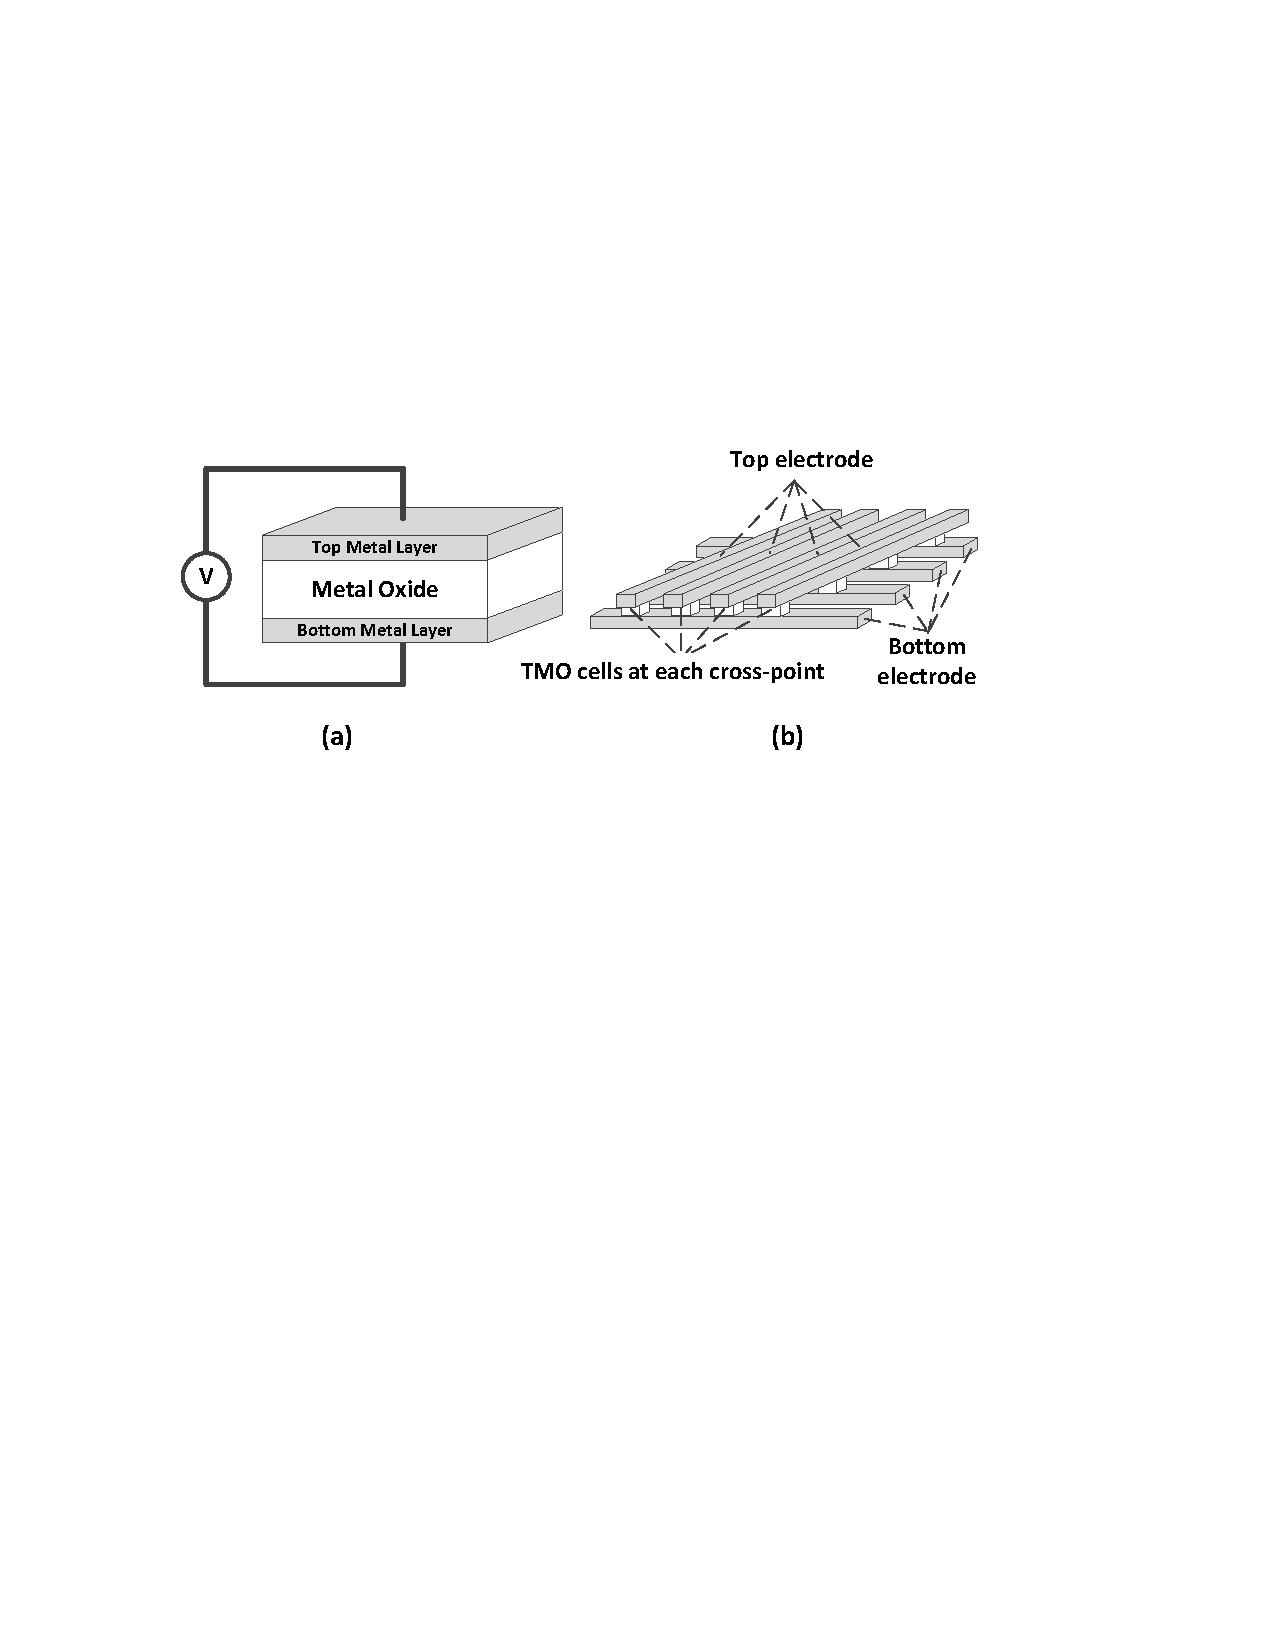
\includegraphics[width=3.3in]{./fig/DATE1.pdf}
\caption{An overview of (a) TMO MIM structure and (b) a cross-point ReRAM array.}
\label{fig:overview}
\end{figure}


\subsection{Memory Structure of ReRAM Array}

Almost all of the random access memories are organized as a matrix-like structure: one memory cell along with its access device (normally a MOSFET) are located in each intersection of horizontal wordlines and vertical bitlines. Similarly, the ReRAM array is also has this NOR-type structure. There are two potential structures of a ReRAM array: the MOSFET-accessed structure (1T1R structure) and the cross-point structure. In the MOSFET-accessed structure, each ReRAM cell has a dedicated MOSFET as its access device. The advantage of this structure is that it is very easy to control each cell in the array independently without crosstalk results from the sneak current in cross-point structure. However, in the MOSFET-accessed structure, the size of the MOSFET should be designed large enough to satisfy the current requirement of the SET/RESET operation. Therefore, the total area of the ReRAM array often determined by the access devices instead of the ReRAM cells, which seriously harmed the area advantage of the ReRAM devices. On the other hand, the cross-point structure is a more area efficient structure compared to MOSFET-accessed structure. As shown in Fig.~\ref{fig:overview}(b), in the cross-point structure, each ReRAM cell is sandwiched by TE and BE at each cross-point of the array without access device. In this structure, each cell only occupy am area of $4F^2$ (F is the feature size of the fabrication technology), which is the theoretical smallest cell area for a single layer single level memory array. For example, Hynix and HP Labs has already demonstrated an 2Mb $4F^2$ cross-point ReRAM chip based on 54nm technology~\cite{TiTa}. In addition, the good 3-D stackability can further reduce the effective cell area. An 64MB $0.5F^2$ cross-point CMOx ReRAM chip was demonstrated by Unity Semiconductor at 2010~\cite{Unity}.


As mentioned, the write operations (SET and RESET) of a ReRAM cell require external voltage across the cell with specified magnitude and duration. To write a cell in the cross-point array, the wordline and bitline where the cell located should be activated at specified write voltage. In addition, all of the unselected wordlines and bitlines are set to a certain voltage or left floating to guarantee that all of the unselected cells are not disturbed. There are several write schemes of the cross-point array. One of the most common scheme for bipolar cross-point array is called HWHB scheme: during the write operation, the selected wordline and bitline are activated at write voltage $V_{write}$ or $0$, while all of the unselected wordlines and bitlines are half biased at $V_{write}/2$. In this scheme, the write voltage $V_{write}$ or -$V_{write}$ is fully applied across the selected cell. The other cells located at the same wordline and bitline with the selected cell are half biased at $V_{write}/2$. And there are no voltage drop across all of the other cells. However, even with proper write schemes, the sneak current at the half selected cells are significant. For a 512x512 array, the sneak current is more than 500 times larger than the SET/RESET current, bring in huge area overhead of the voltage drivers and unnecessary energy consumption at the half selected cells. Therefore, in order to implement a practical cross-point array with acceptable overhead, a large nonlinearity of the ReRAM cell is essential. The resistance of a ReRAM cell with nonlinearity increases with the reducing of applied voltage. In this case, the sneak current at half selected cells will be reduced significantly. The read operation is to bias the selected wordline at $V_{Read}$ and ground all of the other wordlines and bitlines. Then the state of the selected cell is read out by sense amplifier connected to the selected bitline.

%The nonlinearity coefficient is proposed to

Although the cross-point structure suffers from aforementioned
shortcomings, its area efficiency is an attractive superiority compared to other emerging NVMs. In addition, the BEOL CMOS process capability makes it possible to implement the array on top of (part of) the peripheral circuity, further improving the area efficiency. Since the chip area is directly related to the cost-per-bit metric, the cost advantage make the cross-point ReRAM a promising candidate for DRAM or FLASH replacement.


\section{Impact of cell errors on cross-point ReRAM Design}
\label{sec:intro}

Reliability is a vital concern in the design of memory system. In the cross-point structure, the reliability issues comes from two different sources: \emph{\textbf{structural error}} and \emph{\textbf{cell error}}. The structural error comes from the special organization of the cross-point array. The impact of voltage drop, sneak current, write/read schemes, as well as data pattern on the array reliability are well studied in literatures~\cite{jiale,Dimin_ISLPED}. It has been shown that the structural errors can be mitigated or eliminated with exhaustive worst-case design. On the other hand, because of the intrinsic characteristics of ReRAM cells, the impact of cell errors is not avoidable. To implement a reliable ReRAM array, additional detection and recovery mechanisms and circuity are required. In this section, we first discussed the resistance switching behaviors of ReRAM cell. Based on the discussion, mechanisms and modeling of soft error and hard error of ReRAM cell is presented. Then, the impact of the cell errors at the array design is evaluated.

\subsection{ReRAM resistance switching mechanisms}
%A schematic view of the switching mechanisms of ReRAM cell is illustrated in Fig. ~\ref{fig:filament}.
There are several studies have been conducted to reveal the physical mechanisms of the resistance switching behaviors. Recently, the filamentary model is widely accepted to explain the resistance switching phenomenon in the TMOs ReRAM: switchings between LRS and HRS are caused by the formation and rapture of the nanoscale conductive filaments (CFs) at the anode interface of the cell. For forming operation can be considered as a 'preset` operation of the ReRAM cell. The schematic view of the switching mechanisms of ReRAM cell is illustrated in Fig. ~\ref{fig:filament}.

During the forming step, a high voltage is applied across the cell. The dielectric soft breakdown in the materials generates a great amount of the defects in the TMOs, which form one or several CFs through the cell. At the same time, the anode becomes a reservoir of the oxygen ions. After the forming operation, the cell exhibit LRS, which is shown in Fig.~\ref{fig:filament}(a). The RESET operation is shown in Fig.~\ref{fig:filament}(b). In this step, the oxygen ions are forced back to the TMO layer by the electric field and recombine with the oxygen vacancies (Vo). In this case, the CFs are ``cut doff'' and the cell becomes HRS, which is shown in Fig.~\ref{fig:filament}(d). In contrast, the SET operation can be considered as a converse process of the RESET operation. As shown in Fig.~\ref{fig:filament}(c), the SET operation realizes the regeneration of the CFs by separating the oxygen ions and the Vo again. In this case, the cell switches back to the LRS.
\begin{figure}[!t]
\centering
    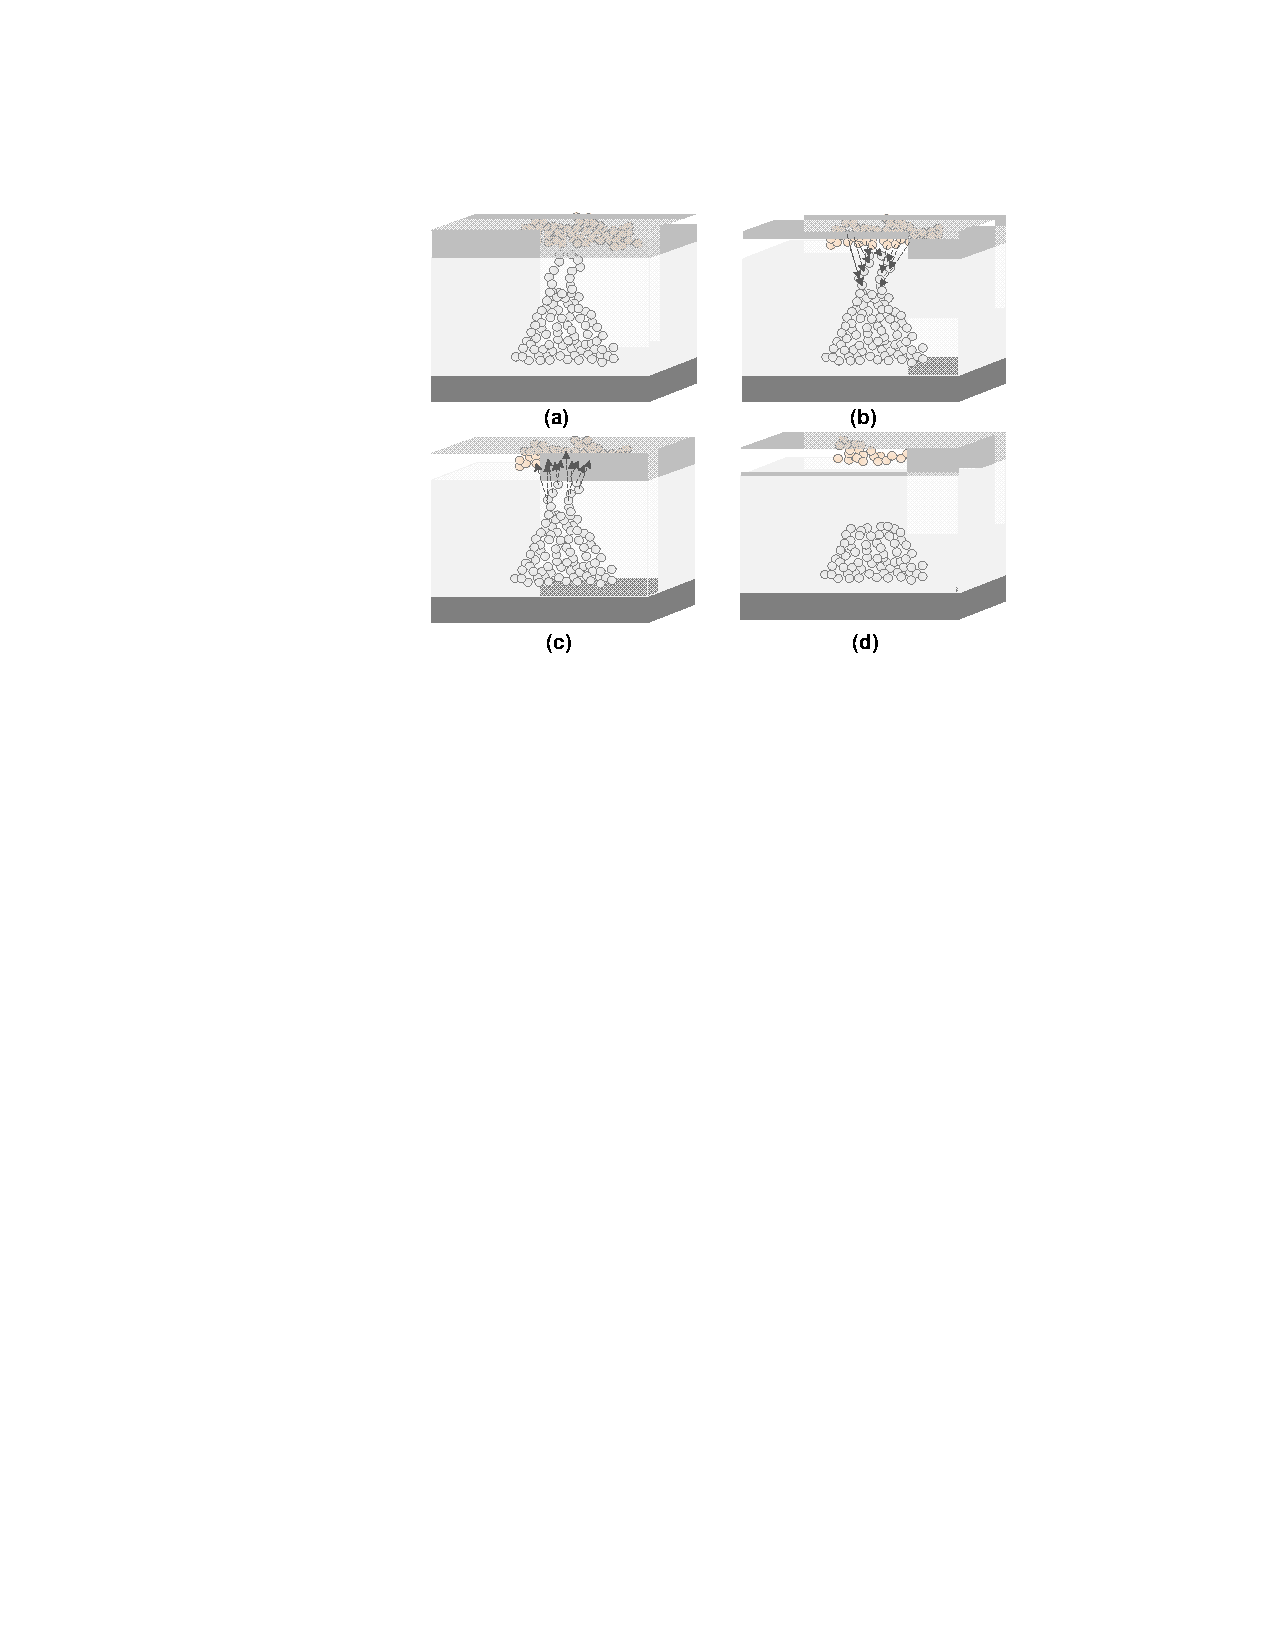
\includegraphics[width=3.5in]{./fig/DATE2.pdf}
\caption{(a) LRS of the ReRAM cell after the formation or SET operation.  (b) RESET operation. (c) HRS of the ReRAM cell after RESET operation. (4) SET operation.}
\label{fig:filament}
\end{figure}

\subsection{Mechanisms and Modeling of Soft Error and Hard Error of ReRAM} \label{sec:Model}

Soft error of the ReRAM cell come from the retention error. The retention failure is a recoverable upset of the resistance of the cell. The retention failure can either be a suddenly resistance drop of the HRS cell (HRS failure) or a suddenly resistance increasing of the LRS cell (LRS failure). The retention failure behaviors result from the random generation of the Vo (HRS failure), and the recombination of Vo with oxygen ions (LRS failure). Both of them imply that the retention failure is a random phenomenon rather than a cumulative phenomenon. Since either of the HRS failure or the LRS failure can be the dominate soft error of the ReRAM with different materials and process technology~\cite{softerror_yu,softerror_gao}, in this paper, we focus on the soft error that dominated by the LRS failure.

In order to quantify the retention failure behavior,the cumulative failure probability is employed. A simplified model of the cumulative failure probability is proposed by Gao~\cite{softerror_gao}, which can be expressed as
\begin{equation}
F(t) = 1-(1-p)^{(\alpha t)},
\end{equation}
where $\alpha$ is a constant value, $t$ is the retention time, ad $p$ is the generation probability of the Vo and has the term of
\begin{equation}
p_H = exp((qVl/2d-\varepsilon_V)/kT),
\end{equation}
where $q$ is the electric quantity if the oxygen ions, $V$ is the applied voltage on the TMO layer, $l$ is the lattice constant, $d$ is the length of the filament's ruptured region, and the $\varepsilon_V$ is the oxygen vacancy's formation energy.

Different from soft error, the hard error results from the limited endurance of the ReRAM cell compared to traditional DRAM/SRAM technologies. The endurance failure is caused by a gradually resistance change over the write cycles. According to different behaviors and physical mechanisms, the endurance failures are classified into three categories~\cite{harderror}:
\begin{enumerate}
  \item Type I Failure: This failure is caused by the generation of extra oxide layer at the anode during the SET operations. This layer prevents the moving of the oxygen ions and results in the increased $R_{LRS}$ and the degreased $R_{HRS}$.
  \item Type II Failure: The programming voltage generated extra Vo, which directly increases the diameter of the CFs. In this failure, both of the $R_{LRS}$ and the $R_{HRS}$ decreases gradually.
  \item Type III Failure:This failure results from the undesired consumption of the oxygen ions at stored in the anode. In this case, the combination probability of Vo and oxygen ions will reduce. Thus the $R_{HRS}$ decreases while the $R_{LRS}$ keeps constant.
\end{enumerate}

\begin{figure}[!t]
\centering
    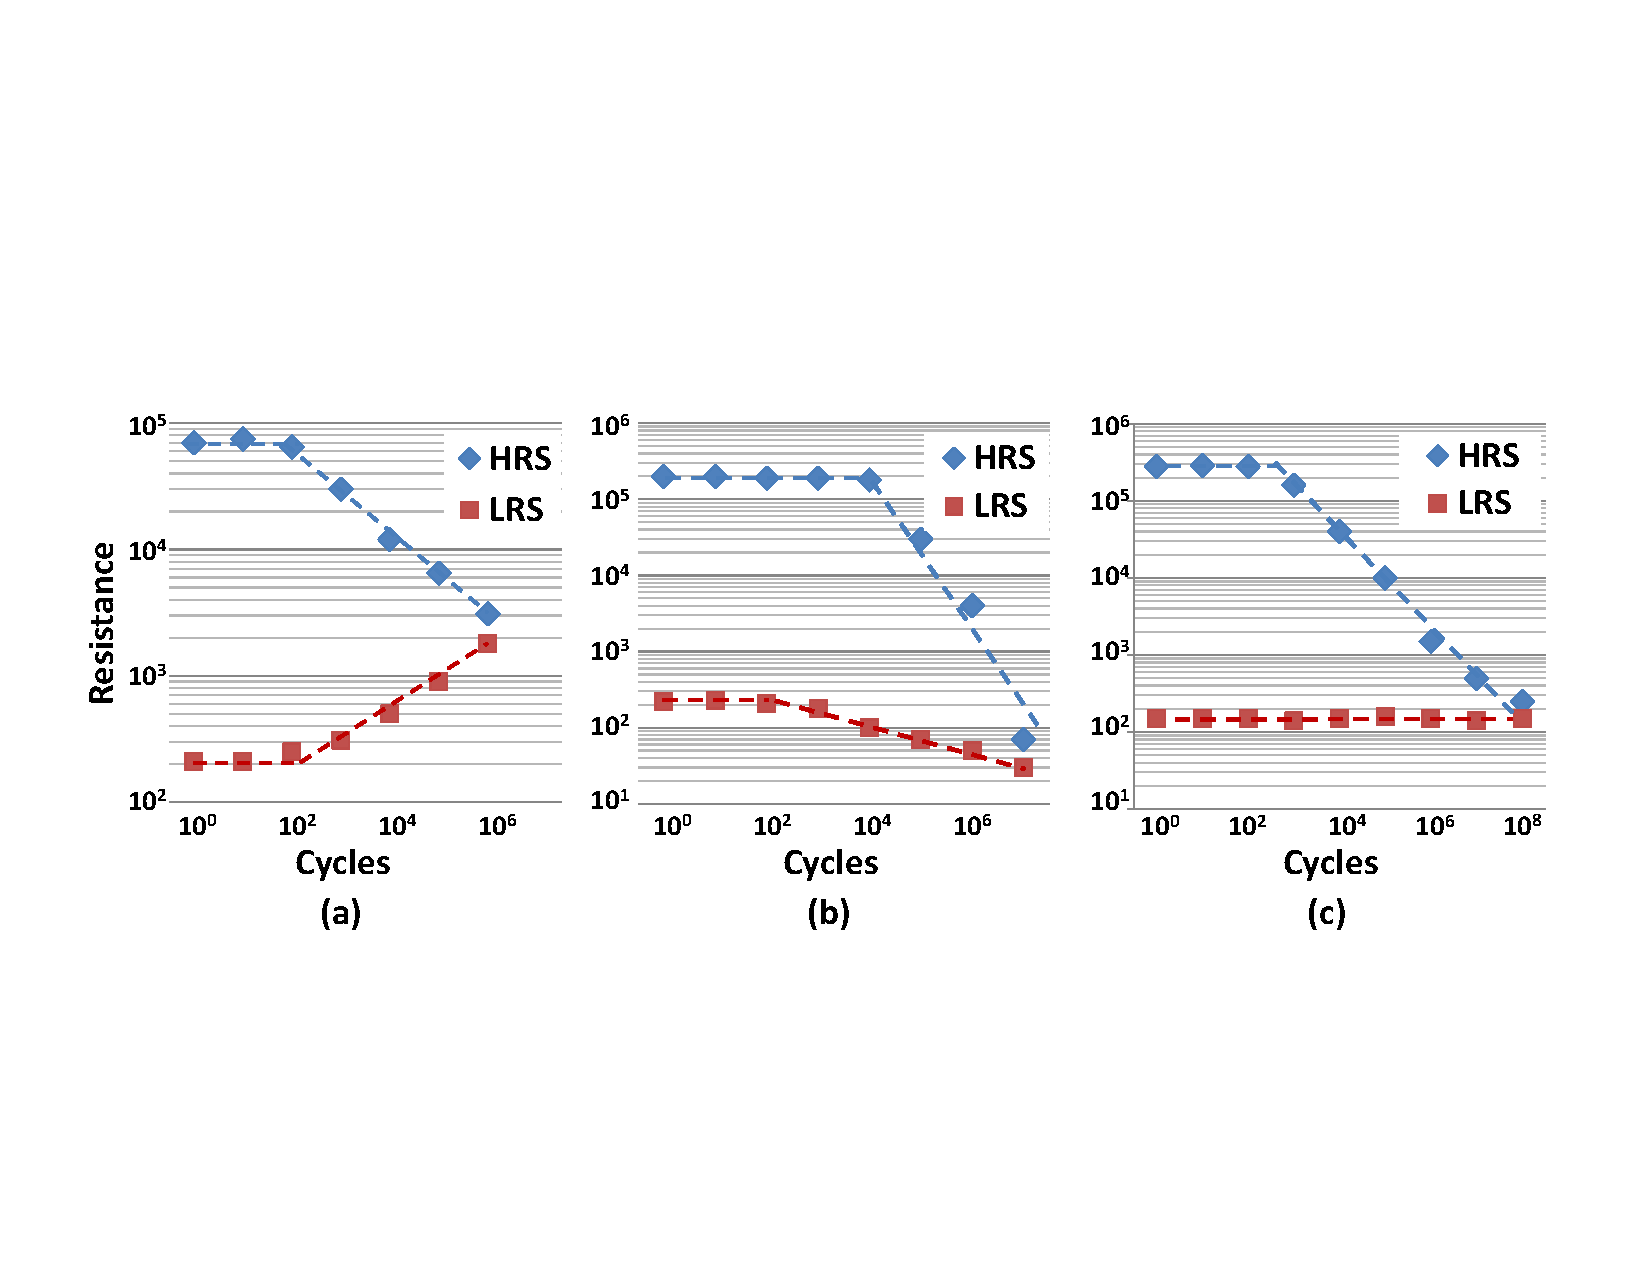
\includegraphics[width=3.5in]{./fig/errors.pdf}
\caption{Hard errors in TMO ReRAM cell: (a) Type I, (b) Type II, and (c) Type III endurance failure.}
\label{fig:errors}
\end{figure}
For simplicity, we proposed a unified model to summarize these three types of endurance failure as
\begin{equation}
R = R_0(1+{\alpha_0(t-t_0)^{\xi}(sgn(t-t_0)+1)/2}),
\end{equation}
where $R_0$ is the initial resistance of LRS or HRS, $t_0$ is the start point that the endurance degradation is observed, and $\alpha_0$ and ${\xi}$ represent the direction and speed of the resistance change. The model with different parameters fits good with the published data and is shown in Fig.~\ref{fig:errors} as dash lines.

\subsection{Impact of Soft and Hard Error on Cross-point Array}
%    512 x 512
%    R_line = 0.65
%    R_h = 500 000;
%    R_l =  20 000;  R_l_half = 100 000;
%    Kr = 10;
%    R_read = 100 000;
%    R_read_h =1 000 000;
The soft error is a recoverable error and represents as a HRS-to-LRS or LRS-to-HRS transition. Therefore, we conclude that soft errors can only affect the information stored in the cells where the endurance failures arise, and will not affect the other cells in the cross-point array. To overcome the soft error, the Error Correction Code (ECC) is necessary. The area, energy, and latency overheads will be evaluate in Section~\ref{sec:expe}.

Compared to the soft errors, the hard errors are more serious, especially for the cross-point structure. In general, the impact of hard errors exists in two aspects: (1) the degradation of the read margin results from the shrink of the resistance ration between the HRS and the LRS. This problem appears in all of three types hard errors; (2) the design overhead that incurred by the hard errors, including the area overhead, energy consumption overhear, as well as more severe array size limitation. However, since the LRS is the decisive for the worst-case design, only the Type II hear error will affect the design.


Fig.~\ref{fig:margin} shows the read margin degradation results from the resistance change of the HRS and LRS. According to the aforementioned Type I-III hard errors, the endurance failures of HRS always represent the resistance reduction. However, the resistance of LRS may either increases (for Type I error) or decreases (for Type II error). Therefore, in this figure, we assume the resistance of HRS can reduce to half of the original value, while that of LRS can either increase or decrease by 50\% of the original value. From the figure, we can see that the reduction of the resistance ratio between HRS and LRS, which results from the resistance increasing of LRS and decreasing of HRS, has significant impact on the read margin. For example, when the resistance of LRS reduces by 50\%, the read margin will reduce by 35\%. And when the resistance of HRS increase by 50\%, the read margin shrinks to only 1.2\% of the original read margin. This observation indicates that the HRS endurance failure brings more serious degradation to the read noise margin. 

%In addition, our simulation also shows that the endurance failures can also make the array unreadable for specific HRS resistance increasing and LRS resistance decreasing. In our simulation, XXXXXXXXXXX Inditace the unreadable region.

\begin{figure}[!t]
\centering
    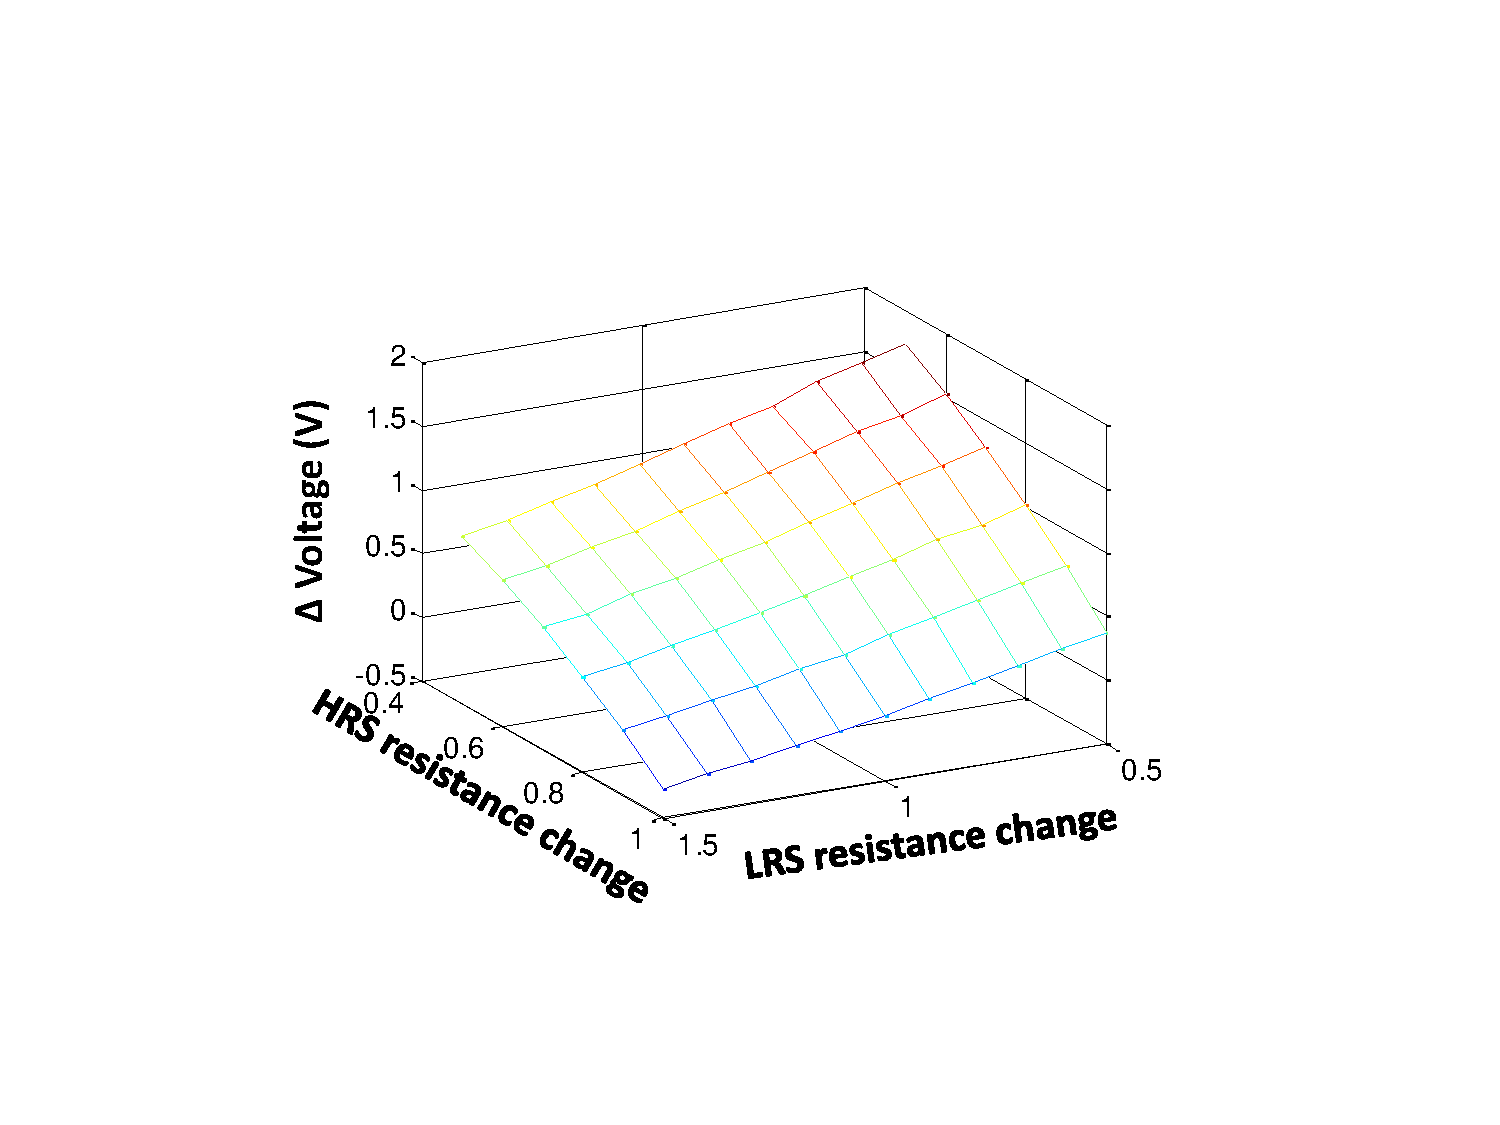
\includegraphics[width=2in]{./fig/margin.pdf}
\caption{Impact of endurance failures on read margin.}
\label{fig:margin}
\end{figure}


As mentioned, to overcome the hard errors, the design limitations of the cross-point array is further deteriorated. To ensure the reliability of the array, the cross-point array is always designed for the worst case - making sure that the array can work reliably, regardless the data pattern in the array. Many researches have been conducted to study the worst case design~\cite{jiale, Dimin_ISLPED} and it has been figure out that the lowest resistance is the key parameter for the worst case design of cross-point array. Since the LRS resistance reduction is only observed in Type II error, therefore, we conclude the Type II hard error is the key player for the worst case design. Firstly, the limitation of the array size results from the voltage drop along the wordlines and bitlines. Our simulation shows that the decrease of the resistance of LRS will aggravate the voltage drop and therefor reduce the allowable array size. As shown in Fig.~\ref{fig:size}, the maximum array size reduces from 512 by 512 to 355 by 355 with the LRS resistance drop to half of its original value. Besides, the energy consumption and the driver current are also impact by the LRS resistance reduction. Fig.~\ref{fig:EC} shows the energy and driver current overhead of the LRS resistance reduction. As shown, the worst case energy consumption of the array increases by 55\%. On the other hand, the driver current in increases up to 72\%. Since the area of the wordline voltage driver and bitline multiplexors is linearly related to the driver current requirement, the area of peripheral circuits are also harmed.


%As mentioned, the existence of the voltage drops along the metal wires and the sneak paths brings in extra reliability issues to the cross-point array design. Firstly, the maximum array size will be reduced due to the hard error. In cross-point array, the

\begin{figure}[!t]
\centering
    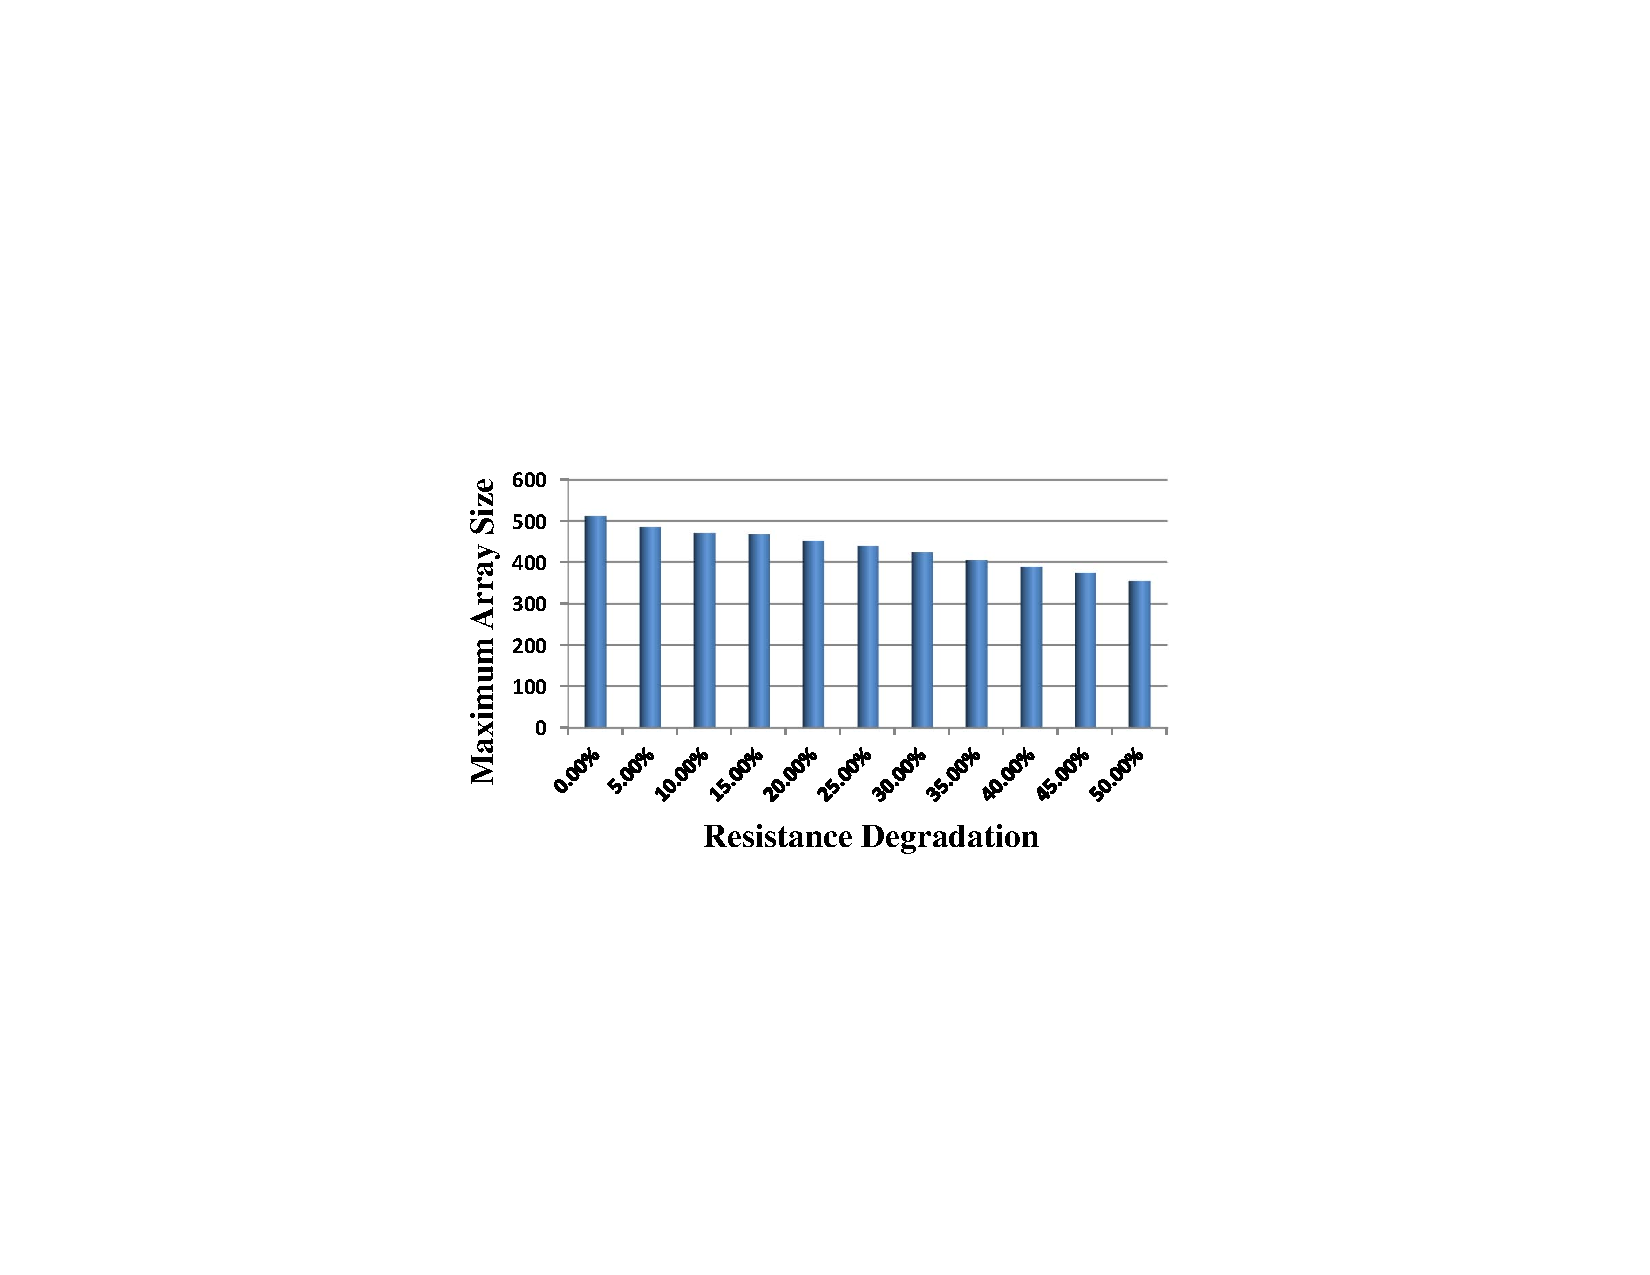
\includegraphics[width=2.5in]{./fig/size.pdf}
\caption{Impact of Type II error on maximum array size.}
\label{fig:size}
\end{figure}

\begin{figure}[!t]
\centering
    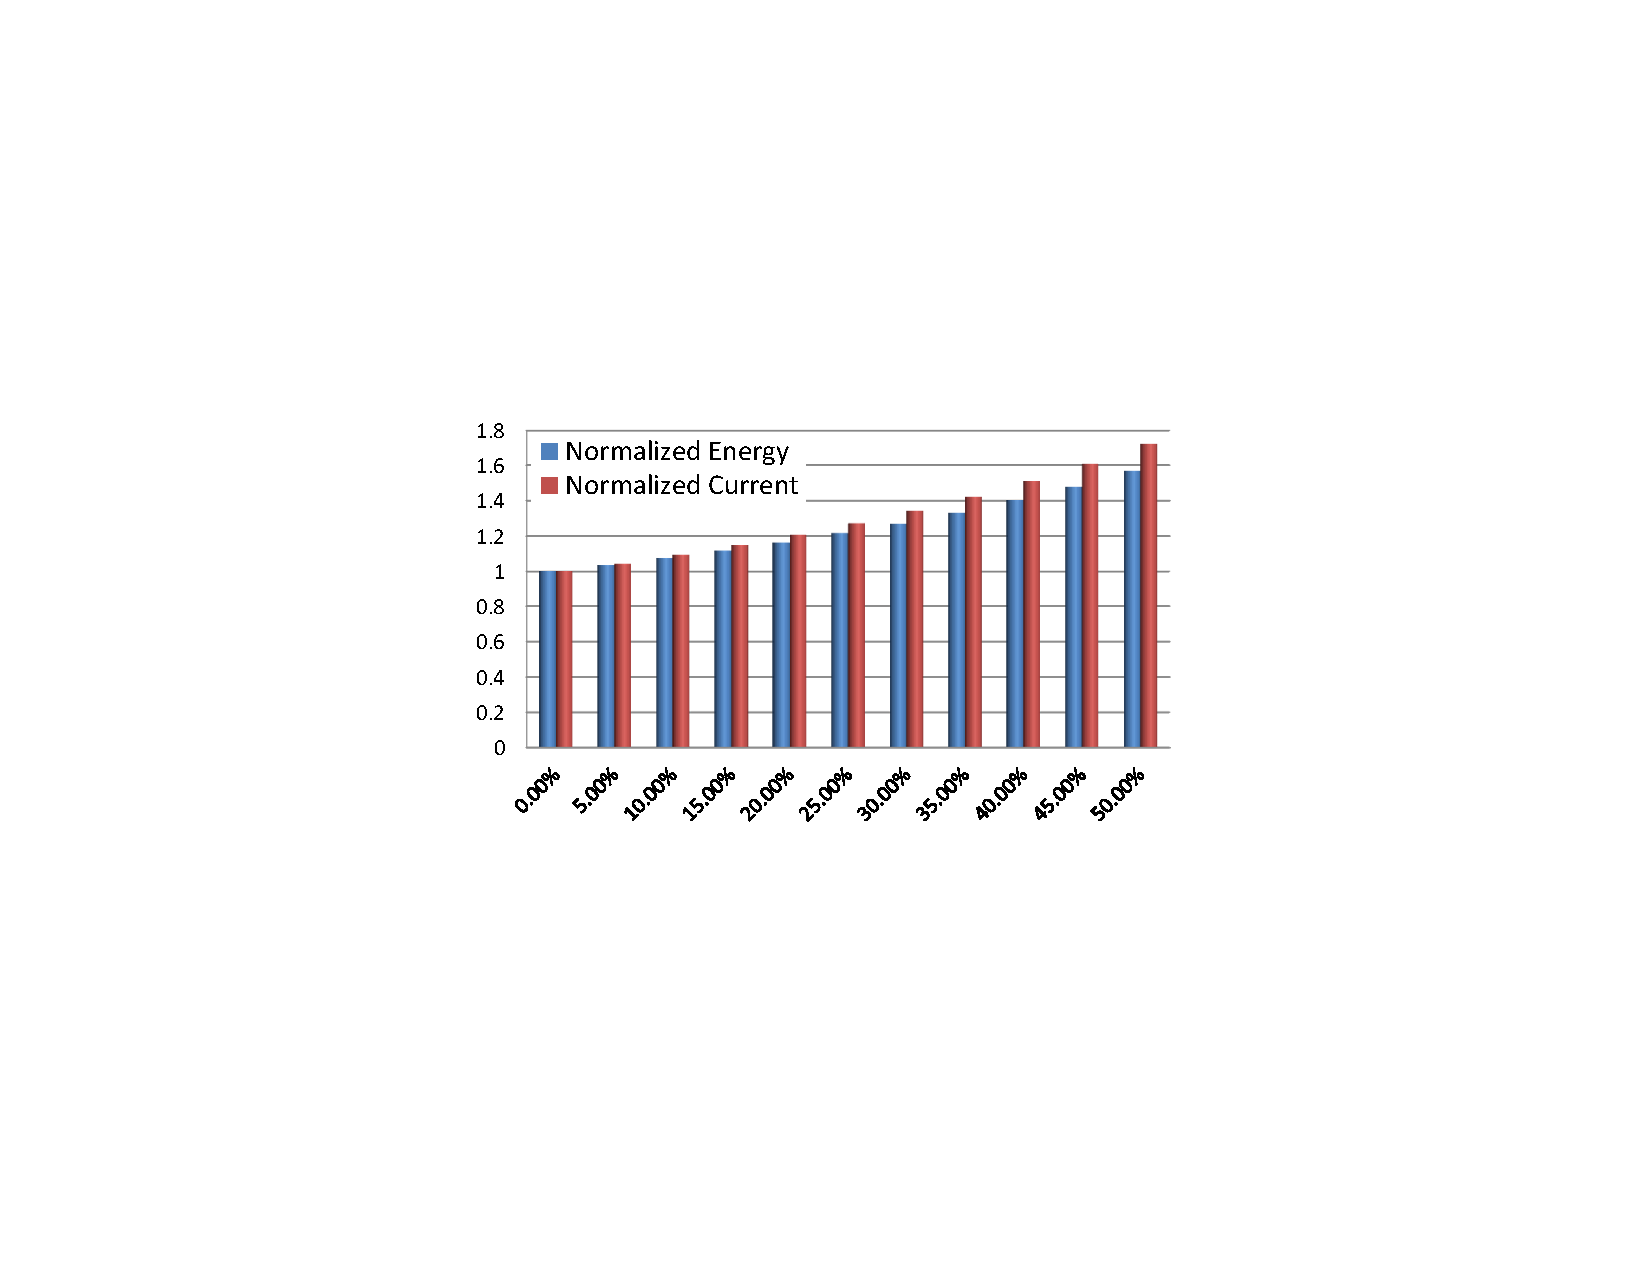
\includegraphics[width=2.5in]{./fig/EC.pdf}
\caption{Impact of Type II error on energy consumption and current requirement.}
\label{fig:EC}
\end{figure}

\section{Soft Error and Hard Error Resilience Design of ReRAM} \label{sec:arch}
A reliable cross-point ReRAM design should be resilient to both of the soft and hard errors. In our design, we proposed a detect-recognize-recover architecture to improve the reliability of the system. The error detection is realized by two-level ECC. The to recognize the error pattern, a multi-level sensing amplifier is applied. According to the error pattern, the recovery mechanisms are achieved either by boosted SET voltage or RESET current.

The proposed soft and hard error resilience design is shown in Fig.~\ref{fig:arch}. Firstly, a block-failure-table (BFT) is proposed to record the failure block and the failure behaviors of the block. As shown in Fig.~\ref{fig:arch}(b), the BFT is implemented as a content-addressable memory (CAM). Each entry in the table contains the physical address of the block, a HRS failure bit (HFB), and a LRS failure bit (LFB). Before every write operation, the BFT is checked to recognize if the hard errors has already appears at the accessed block. In order to mitigate the performance degradation and to guarantee the reliability, the BFT is implemented as a 1T1R structure. The number of the entries in the BFT directly affects the failures tolerance of the proposed architecture: although a larger BFT can record more failure blocks in the memory, the area and latency overhead will also increase significantly.


\begin{figure}[!t]
\centering
    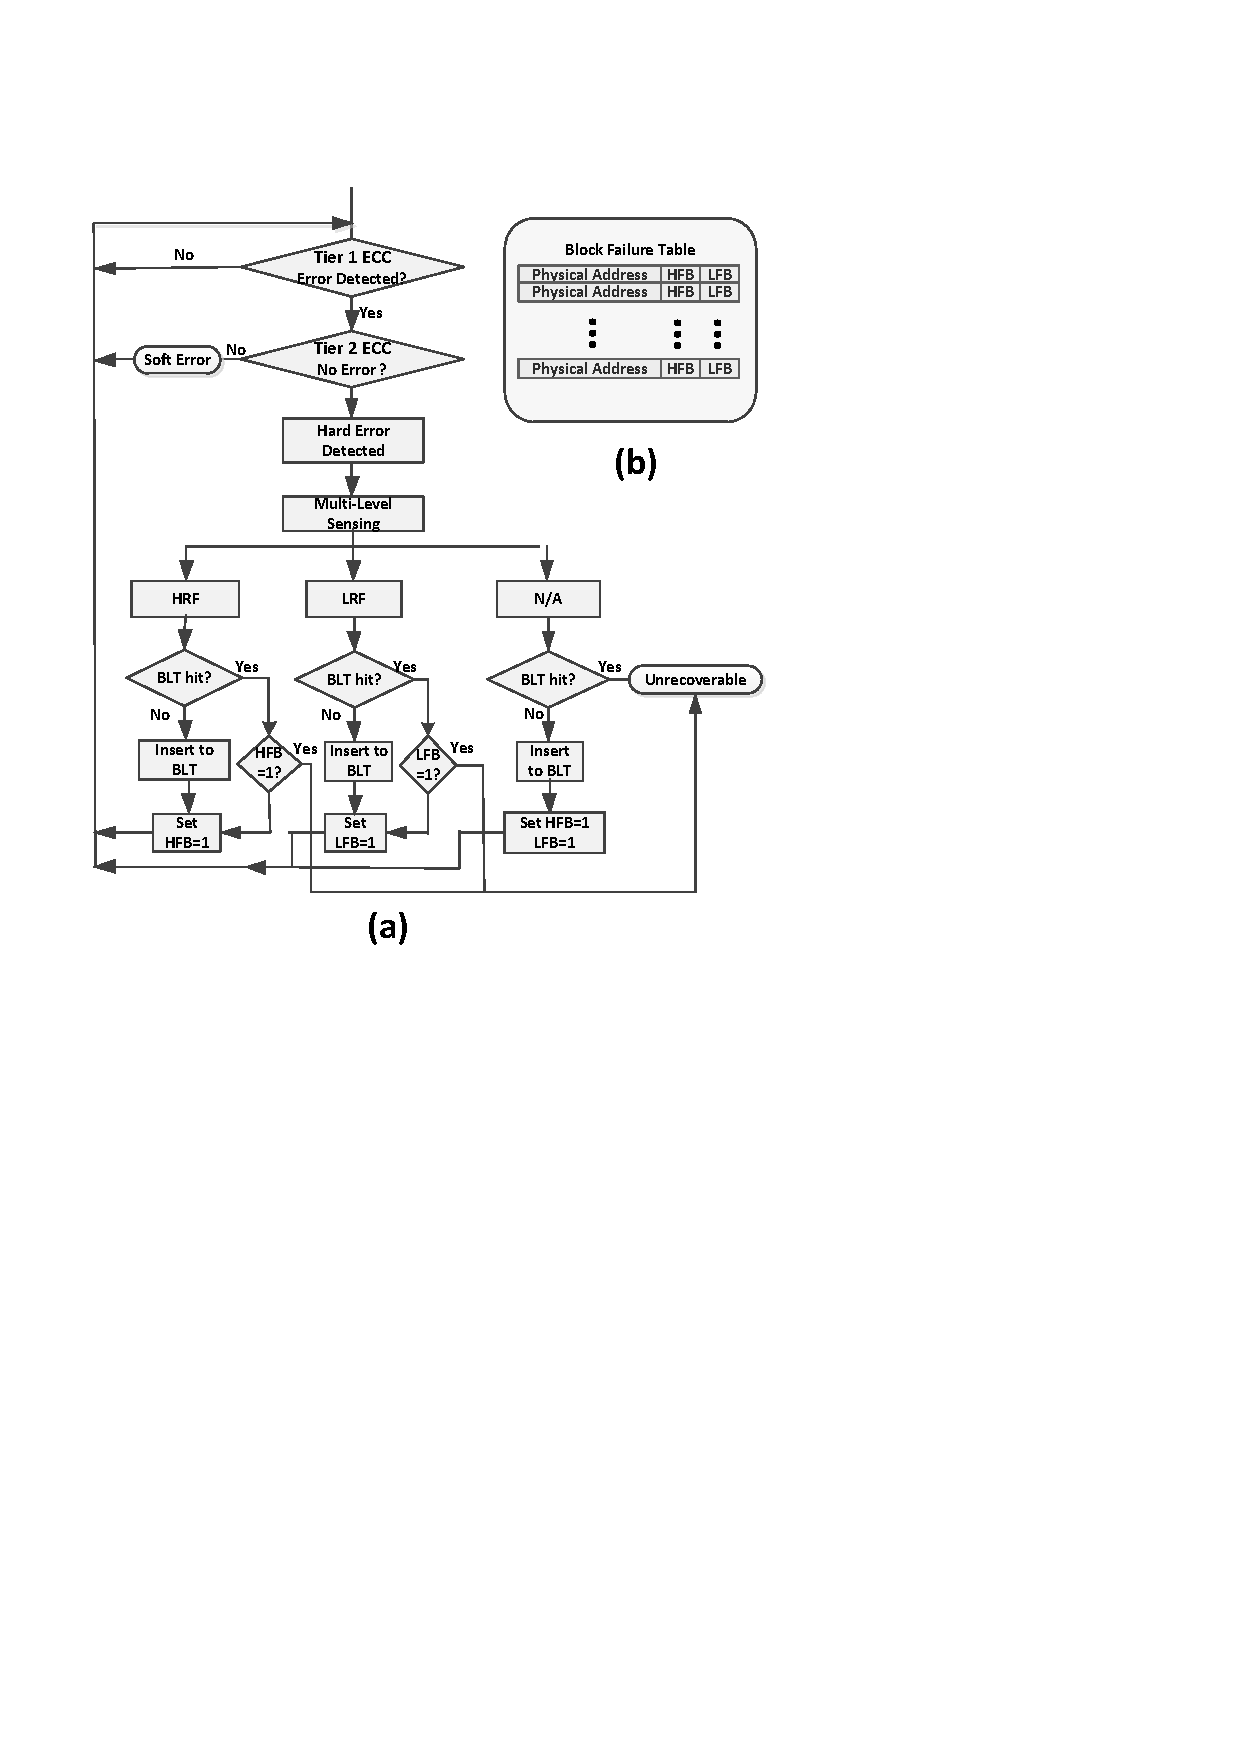
\includegraphics[width=3.4in]{./fig/arch.pdf}
\caption{(a) Soft and Hard Error Resilience Design. (b) BFT organization.}
\label{fig:arch}
\end{figure}

\begin{figure}[!t]
\centering
    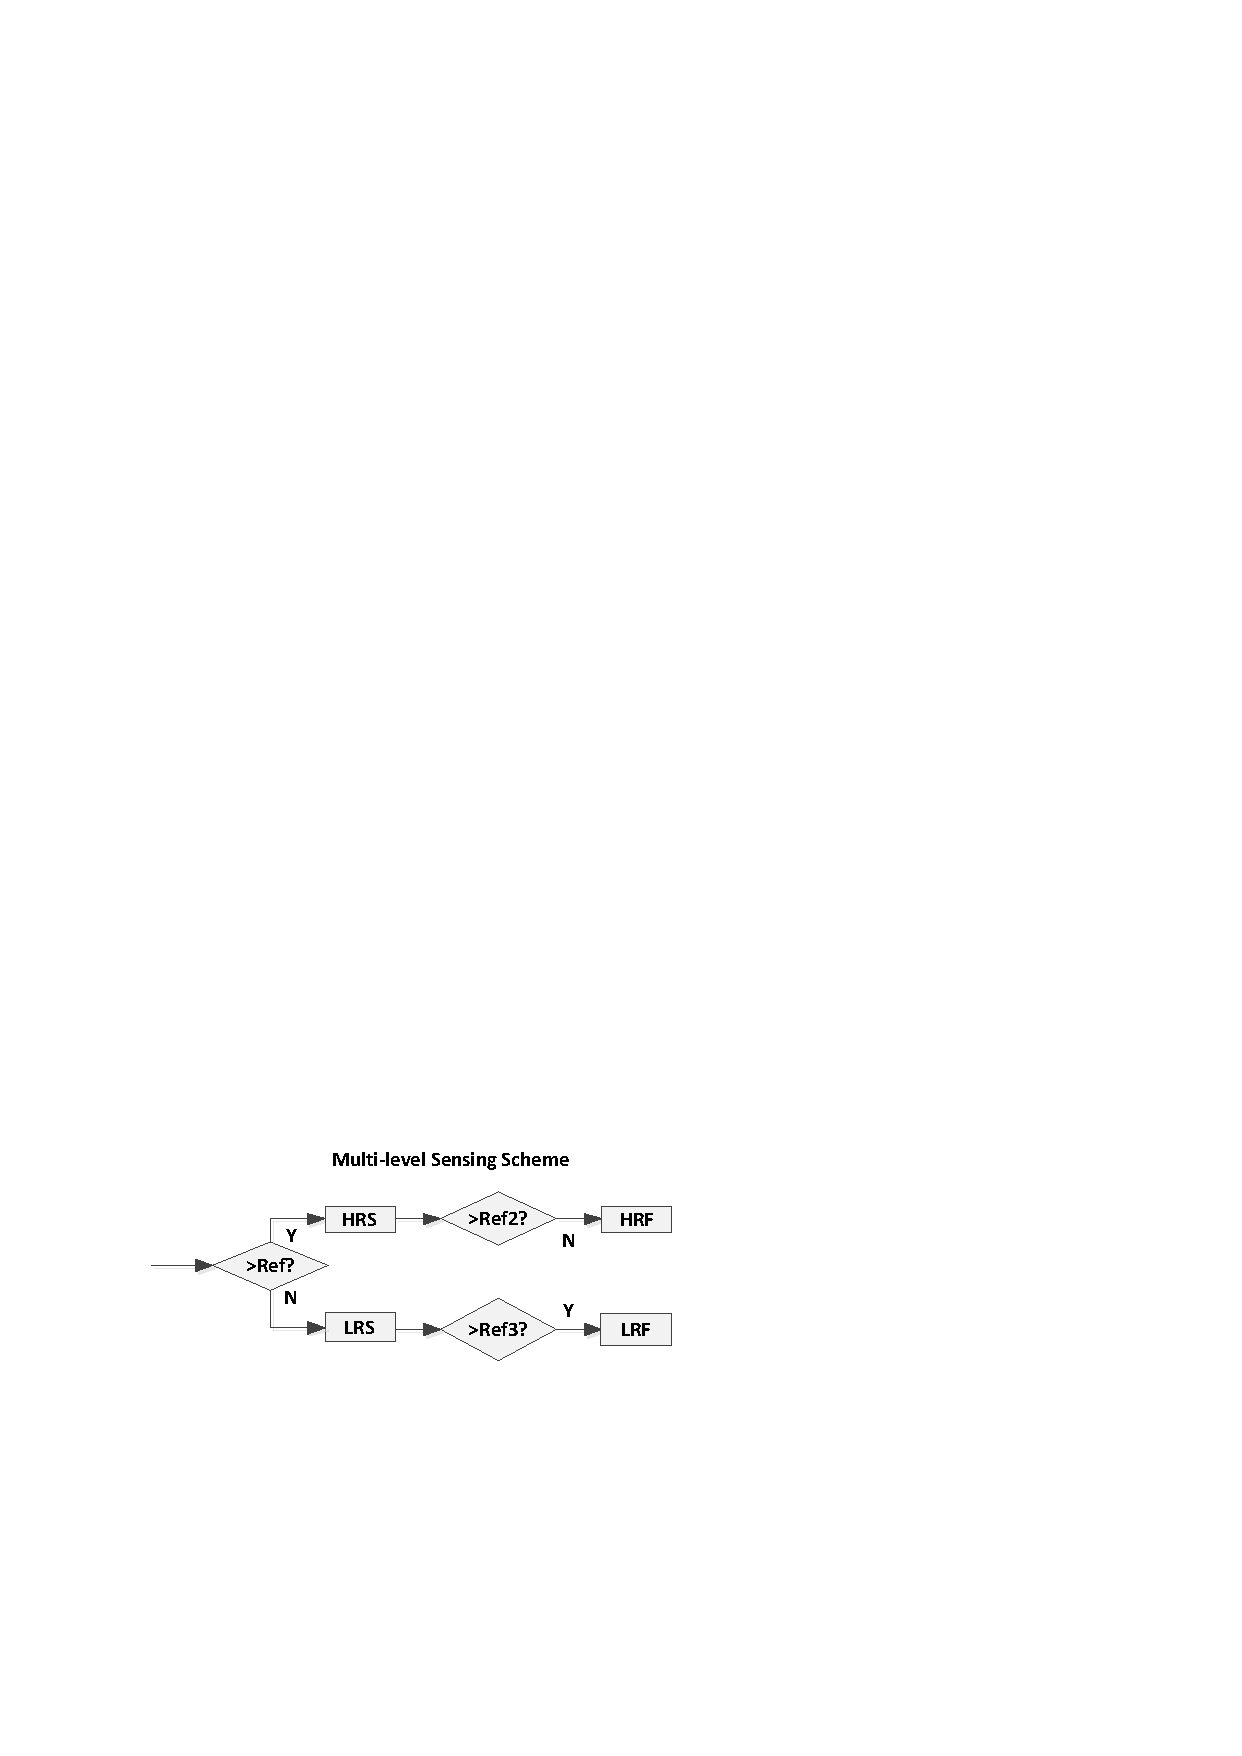
\includegraphics[width=3in]{./fig/sense.pdf}
\caption{Multi-level sensing scheme.}
\label{fig:sense}
\end{figure}

%In addition, the purpose of the proposed architecture is to detect the failure at a early stage and ensuring the system operate correctly at the same time.

The detection part is realized by two-level ECC: the first level ECC is a simple SEC-DED code, dealing with the soft error; the second level ECC is more complex with multi-bit correcting capability, which can detect and correct the errors results from the initial retention failure bits. If the first ECC level shows that no error detected, no further action is required. However, if the error is detected at the first level ECC, the data is sent to the second layer ECC. As soon as the multi-bit error is detected by level-2 ECC, the retention failure is confirmed. 

Simultaneously, the multi-level sensing is triggered to recognize the error pattern. As shown in Fig.~\ref{fig:sense} , the multi-level sensing can be used to distinguish the HRS failure and LRS failure. According to the output of multi-level sensing circuity, the corresponding bit (HFB or LFB) is updated. If the HFB or LFB is already been marked, the block is considered as a unrecoverable block and further replace action is required. Otherwise, the recover mechanisms will be performed during the following write operation to this block.

 


\section{Experimental Results} \label{sec:expe} 
\section{Conclusion} \label{sec:conc} 

\scriptsize
\bibliographystyle{unsrt}
\bibliography{date2012}

\end{document}


